\documentclass{article}
\usepackage[utf8]{inputenc}
\usepackage{graphicx}
\usepackage{hyperref}
\setlength{\parskip}{1em}
\title{CS376 Term Project}
\author{Team 16}

\begin{document}
\maketitle

\section{Model Descriptions}

% Provide descriptions about your model components, algorithms and applied methods.
% You should use figures and equations for clear descriptions.
% Only text descriptions will lose points.

We mainly used \textit{XGBoost} to learn the data. XGBoost is a popular gradient boosting library that offers efficient supervised learning. We chose XGBoost because our TAs suggested it during the TA sessions and it is widely used among Kaggle winners.

XGBoost internally uses \textit{decision tree ensemble}. When we train model, it classifies the data with multiple trees and based on decision, it gets score. Then based on the loss, it learns the tree weights. For instance, example below illustrates how multiple decision trees work to predict house price of the Gotham city.

\begin{figure}[h]
\centering
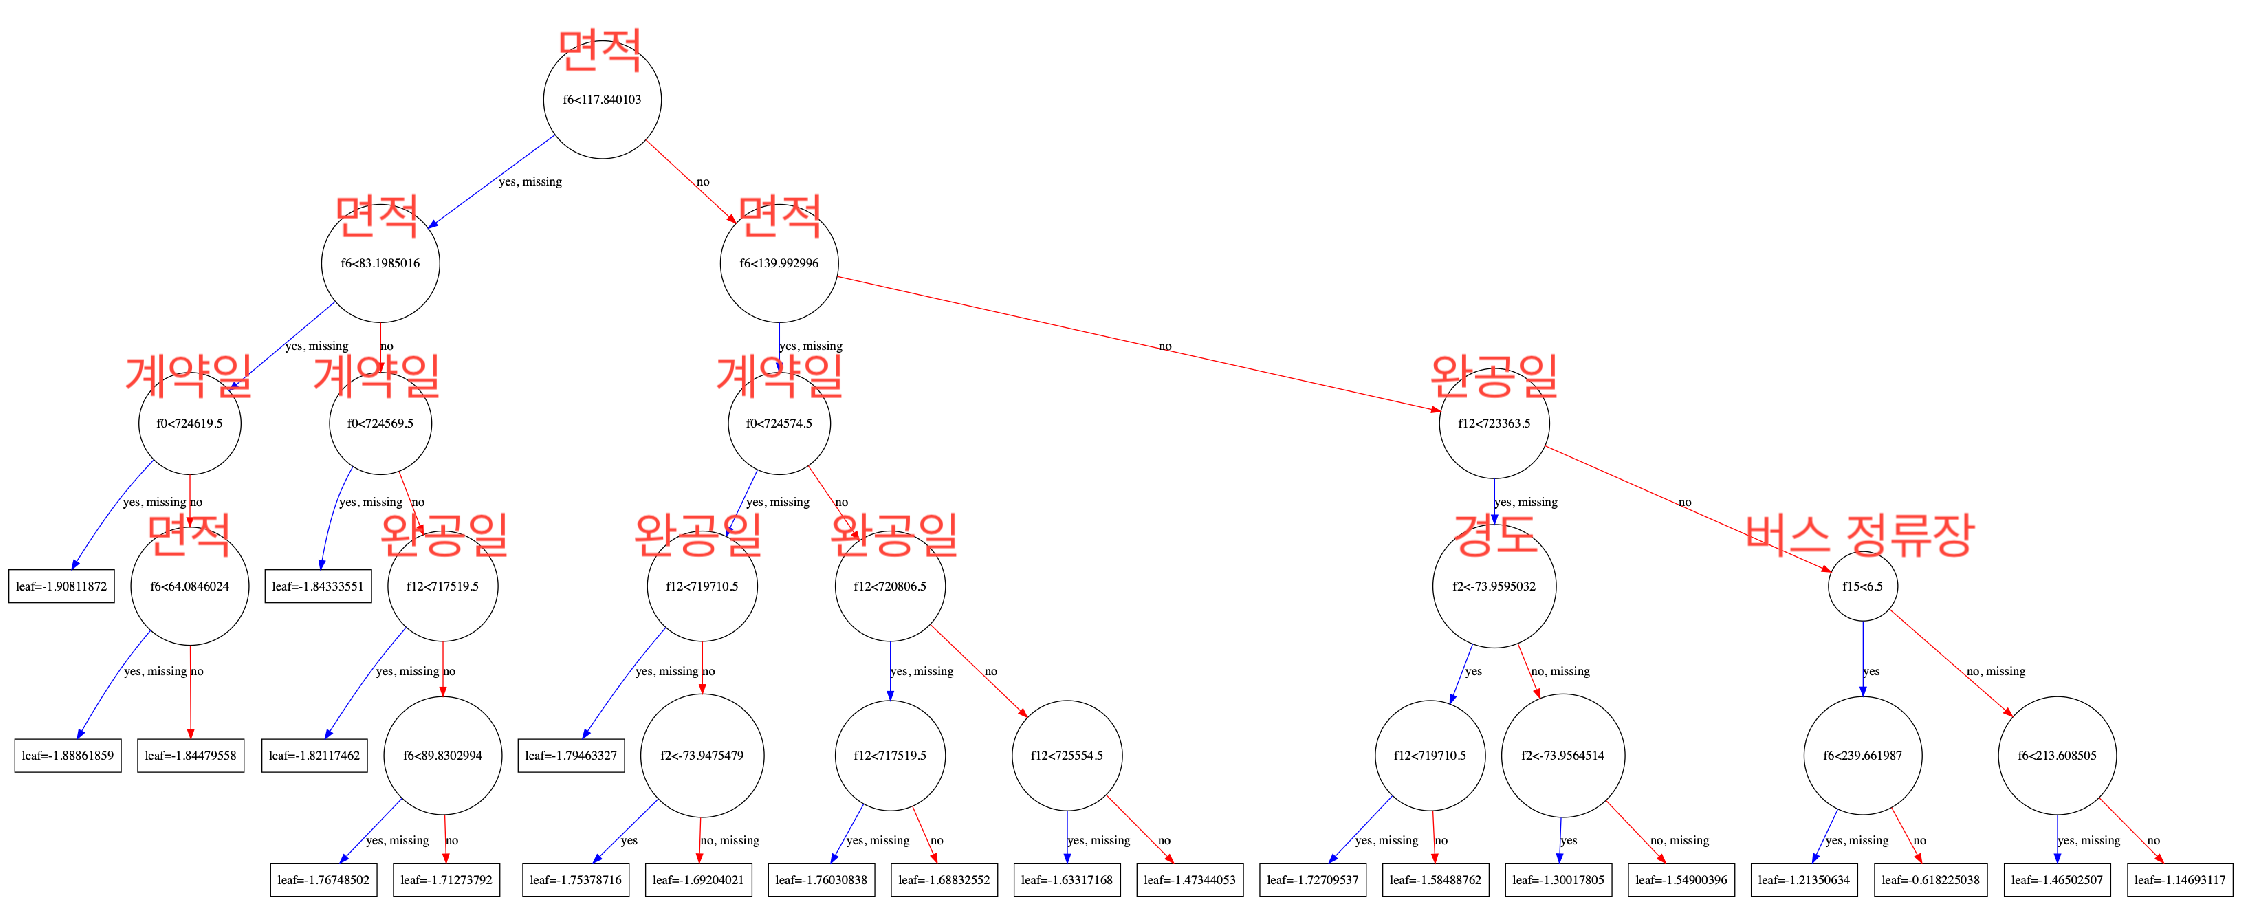
\includegraphics[width=1\textwidth]{Depth5}
\caption{Example of boosted tree}
\end{figure}

For preprocessing, we first read the data with \textit{pandas}. We replaced two date types \textit{contract date}, \textit{completion date} into three columns each: \textit{year}, \textit{month}, \textit{day}. We shuffled the data to reduce variance and avoid overfitting. We intentionally let the missing values intact for the base model, because XGBoost handles missing values appropriately; it learns how to treat missing values in each boosted tree.

We tuned the hyper-parameters including \textit{max depth of the boosted tree} and \textit{number of iterations}.

\section{Unique Method}

% In the below subsections, state applied methods that you think unique and why

\subsection{Drop outliers}
We first carefully investigated whole dataset and found that there's outliers. We decided to drop records with price larger than 450,000 and altitude less than 30, i.e.,

$$ price >= 450000 \lor altitude < 30 $$

\subsection{Drop unrelated columns}
We dropped \textit{completion month}, \textit{completion day} as they are always january first. Also we deleted following columns as it seemed they are not contributing to the accuracy of final model.

\begin{itemize}
	\item Altitude
	\item Road id
	\item Apartment id
	\item Whether an external vehicle can enter the parking lot
	\item The number of households in the apartment
	\item Average age of residents
	\item The number of schools near the apartment
	\item The number of bus stations near the apartment
	\item The number of subway stations near the apartment
\end{itemize}

One may find that many of them are categorical data. To handle categorical data, we first tried \textit{one-hot encoding} from \textit{scikit-learn}, but some of the columns make training take too much time while it doesn't contribute to the accuracy. When we made over 1400 columns, the process crashed as it uses too much memory. So we removed categorical data with too many values: \textit{road id} and \textit{apartment id}

\subsection{Handling missing data with Imputer}
We applied different missing value filling strategy to each columns. For instance, we filled \textit{area} with mean value, and \textit{builder id} with 0.

\section{Libraries}

% Specify libraries with versions used in the code.
% Describe purposes of the libraries.

\subsection{Pandas}
Version: 0.23.4 \\
Purpose: To efficiently read data with appropriate labels.

\subsection{xgboost}
Version: 0.81\\
Purpose: To learn model with decision tree ensemble

\subsection{matplotlib}
Version: 3.0.2 \\
Purpose: To visualize the data

\subsection{scikit-learn}
Version: 0.20.0 \\
Purpose: To fill the missing values with \textit{Imputer}, and \textit{one-hot encode} the categorical data.

\subsection{numpy}
Version: 1.15.4 \\
Purpose: To conveniently manipulate matrices.

\section{Source codes}

% You should describe
% 1. Which parts in the codes correspond to the model components.
% 2. Which parts are for the test and how TAs can test with another test set.
% 3. Hyper-parameters to use for test.

Git repository: \url{https://github.com/YujinGaya/ml-term-project/}

To inspect what we did, you only need to see \textit{base.py} and \textit{unique.py}.
Following explanation is about the unique method. All the line numbers are line number of unique.py we submitted.

\textit{data\_setting()} function is to load and preprocess data, \textit{performance()} is to measure the performance based on the criteria. and \textit{train\_n\_predict()} is used to train the model and predict \^{y} for train and test dataset. \textit{main()} calls the three functions appropriately.

If you want to test our source code with another train and test sets, you can edit the parameter of the \textit{pd.read\_csv()} call in line 30 to appropriate file name and train and test. Alternatively, if you only want to test our model without training it with new training set, you can just load the .model files

We tuned \textit{depth of boosted tree} with \textit{max\_depth} parameter in line 147, \textit{number of iterations} with third positional parameter of the \textit{xgb.train()} in line 153.

\section{Performance}
% Report your performance and analyze it. You should specify
% 1. How you split the samples in train data for training and validation.
% 2. Performances on the training and validation samples.
% 3. Execution time on test data.
% 4. Analysis of the performance.

We splitted the samples into 9:1 after shuffling the dataset. We used 9 part to train the model, and 1 part to validate.

For training set, performance of base model is \textit{0.944927}, and performance of unique model is \textit{0.950915}.

For validation set, performance of base model is \textit{0.942786}, and performance of unique model is \textit{0.948572}.

It takes 1 minute to train base model, 4 minutes to train unique model in the VM with 4 cores without CUDA (what we provided from the class).

Since there's not much difference between the performance from the training set and validation set, we think our model is not overfitted.
\end{document}